\section{Competition}
The task that was given was to solve the sokoban puzzle on a map put in the foyer of the Mærsk Mc-Kinney Møller building on SDU, as fast as possible.
The entire course was given the same task, and the group with the fastest time won a prize.
The map is composed of lines, and intersections, where the intersections are to be considered as spaces in the sokoban map. 
A representation of the map can be seen in figure \ref{fig:comp_map}.
One of the things to note is that the foyer has glass walls and the competition is at noon, which means that the sun can play a role.

\begin{figure}[H]
 \centering
 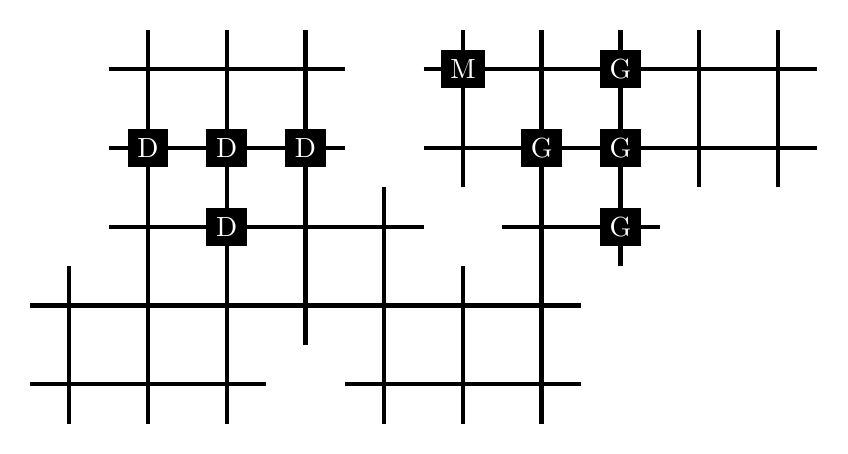
\begin{tikzpicture}
 \draw[ultra thick] (0,0) to (0,2);
 \draw[ultra thick] (1,0) to (1,5);
 \draw[ultra thick] (2,0) to (2,5);
 \draw[ultra thick] (3,1) to (3,5);
 \draw[ultra thick] (4,0) to (4,3);
 \draw[ultra thick] (5,0) to (5,2);
 \draw[ultra thick] (5,3) to (5,5);
 \draw[ultra thick] (6,0) to (6,5);
 \draw[ultra thick] (7,2) to (7,5);
 \draw[ultra thick] (8,3) to (8,5);
 \draw[ultra thick] (9,3) to (9,5);
 
 \draw[ultra thick] (-0.5,0.5) to (2.5,0.5);
 \draw[ultra thick] (3.5,0.5) to (6.5,0.5);
 \draw[ultra thick] (-0.5,1.5) to (6.5,1.5);
 \draw[ultra thick] (0.5,2.5) to (4.5,2.5);
 \draw[ultra thick] (0.5,3.5) to (3.5,3.5);
 \draw[ultra thick] (0.5,4.5) to (3.5,4.5);
 \draw[ultra thick] (5.5,2.5) to (7.5,2.5);
 \draw[ultra thick] (4.5,3.5) to (9.5,3.5);
 \draw[ultra thick] (4.5,4.5) to (9.5,4.5);
 
 \node[draw,fill,text=white] at (5,4.5){M};
 \node[draw,fill,text=white] at (2,2.5){D};
 \node[draw,fill,text=white] at (3,3.5){D};
 \node[draw,fill,text=white] at (2,3.5){D};
 \node[draw,fill,text=white] at (1,3.5){D};
 \node[draw,fill,text=white] at (6,3.5){G};
 \node[draw,fill,text=white] at (7,3.5){G};
 \node[draw,fill,text=white] at (7,4.5){G};
 \node[draw,fill,text=white] at (7,2.5){G};
 \end{tikzpicture}
 \caption{Map as it was put up in the foyer, without the black boxes however. They are merely to illustrate where the goals and diamonds are positioned}
 \label{fig:comp_map}
\end{figure}

